\documentclass[twoside]{article}
\input{ISC18-english.sty}
%%%%%%%%%%%%%%%%%%%%%%%%%%%%  Make sure to compile twice for proper cross-references. %%%%%%%%%%%%%%%%%%%%%%%
%%%%%%% For proper display of references, compile the document twice. %%%%%%%%%%%%%%%%%%%%% 
%%%%%%%%%%%%%%% If using TeX Live, compile using pdflatex command %%%%%%%%%%%%%%%%%%%%%%%
\begin{document}
\thispagestyle{empty}
%%%%%%%%%%%%%%%%% Article title header  %%%%%%%%%%%%%%%%%%%%
\fancyhead[LE]{Analysis of Persian Legal Document Networks...}
%%%%%%%%%%%%%%%%% Article authors header   %%%%%%%%%%%%%%%%%%%%
\fancyhead[RO]{M. Farhadishad \& M. Khansari}
\begin{center}
{
\includegraphics [height=25mm, width=150.3mm] {Images/isc18E}} \\
\vspace*{-1.8cm}
%\begin{center}
%\color{blue} 
%{\hspace{0.1cm}\rule{\textwidth}{1mm}}\\
%\end{center}
\vspace*{4cm}
%%%%%%%%%%%%%%%%% Article title  %%%%%%%%%%%%%%%%%%%%
{\Large \bf Analysis of Persian Legal Document Networks Using Complex Network Techniques and Natural Language Processing}\\
%%%%%%%%%%%%%%%%% Article authors and affiliations %%%%%%%%%%%%%%%%%%%%
{\bf
Mohammad Farhadishad$^1$, Mohammad Khansari  \footnote[2]{{\bf Corresponding Author:} {\tt m.khansari@ut.ac.ir }} \\
$^1$1 PhD Student of Information Technology Engineering, Department of Data Science and Technology
Faculty of Intelligent Systems, College of Interdisciplinary Science and Technologies, University of Tehran
Tehran, Iran
 \\
$^2$PhD, Associate Professor, Faculty Member,
Faculty of Intelligent Systems, College of Interdisciplinary Science and Technologies, University of Tehran
Tehran, Iran
}
\end{center}
\rule{\textwidth}{0.2mm}\\
%%%%%%%%%%%%%%%%% Article abstract  %%%%%%%%%%%%%%%%%%%%
\noindent{\bf Abstract:}\\
Many real-world systems can be effectively modeled and analyzed using graph-based approaches. Despite the growing interest in legal network analysis, studies on Persian legal networks remain limited, particularly those integrating complex network science and artificial intelligence. This study investigates a large-scale Persian legal network constructed from 4,921 judicial rulings, 15 charge titles, and 807 legal documents from the criminal courts of the Islamic Republic of Iran. While the original dataset contained only judicial rulings, charge titles and legal documents were automatically extracted from ruling texts using natural language processing and an AI-based question-answering model. The extracted entities were used to construct and analyze bipartite and tripartite legal networks. Results show that the network exhibits several structural properties commonly observed in real-world complex networks. Furthermore, the proposed multi-level representation reveals meaningful relationships among judicial rulings, charge titles, and legal documents, providing valuable insights for legal network analysis.
 
\noindent{\bf Keywords:} 
Complex networks, multipartite graphs, legal networks, natural language processing, intelligent question and answer. \\
\noindent{\bf Mathematics Subject Classification (2010):} $\rm 99X99$, $\rm 99X99$, $\rm 99X99$. \\
\hspace{1cm}\rule{\textwidth}{0.2mm}\\
%%%%%%%%%%%%%%
\section{Introduction}
\subsection{	Introduction to Intelligent Question and Answer Systems}

Answer selection is a key task in information retrieval and NLP that ranks candidate answers by relevance to a given question \citep{Yih:2013,Chen:2018a}. Earlier methods used static embeddings such as GloVe and Word2Vec, but these models could not fully capture contextual meaning \citep{Pennington:2014,Mikolov:2013,Chen:2018b}. Transformer-based models, particularly BERT, address this limitation through contextual representations and have outperformed feature-based and RNN-based approaches in answer selection tasks \citep{Devlin:2019,Vaswani:2017,Kamath:2019,Severyn:Moschitti:2013,Chen:2017,Rao:2016,Tay:2017,Rao:2019,Liu:2019}. However, challenges remain regarding domain-specific use and insufficient test-data coverage \citep{Devlin:2019,Mayhew:2020}.

\subsection{Introduction to Complex Networks}
Many real-world systems can be represented and analyzed using graph theory, including actor networks, co-authorship networks, and other social, biological, and technological systems \citep{Watts:Strogatz:1998,Newman:2001,Laskar:2019}. Research has shown that diverse networks share common structural properties such as heterogeneous degree distributions, high clustering coefficients, and short path lengths \citep{Watts:Strogatz:1998}. Consequently, complex network analysis has been widely adopted across disciplines including computer science, biology, economics, linguistics, and social sciences. More recently, these methods have also been applied to legal systems, enabling the modeling and analysis of legal networks and their underlying relationships \citep{FoschVillaronga:2022,Gordon:2021,Boulet:2011,Bourcier:Mazzega:2007}.

\section{	Problem statement   }
This study investigates the application of complex network science to Persian legal analysis through a large-scale legal network composed of judicial rulings, legal documents, and charge titles. Traditional representations based solely on judicial rulings and citation links are insufficient to capture the hierarchical and multi-level nature of legal systems, where direct and indirect interactions among rulings, legal documents, and charge titles jointly influence legal processes. To model these layered relationships, this study employs simple directed, bipartite, and tripartite graph structures. Bipartite graphs, which partition nodes into distinct sets connected by inter-set links, have proven effective for analyzing \citep{Siqueira:2026,Ahn:2011,Tumminello:2011} and modeling \citep{Siqueira:2026,Gong:Luo:2025,Tarissan:2013,Guillaume:Latapy:2004} complex networks by revealing structural patterns that may remain hidden in conventional graph representations. Using these network models, we extract and analyze key structural characteristics of the Persian legal network.

\section{	The Proposed Method }

\subsection{ Training Dataset for the Intelligent Question and Answer System}
The training dataset consisted of 9,800 general Persian texts, 250 legal texts, and 200 judicial rulings annotated with questions related to cited legal articles and charge titles. In total, the dataset included 10,250 documents and more than 100,000 question-answer pairs.

\subsection{Modeling the Intelligent Question and Answer System}
A Multilingual-BERT model was fine-tuned for the question-answering task using a learning rate of $2\times 10^{-5}$, a batch size of 16, and three training epochs. The annotated dataset was divided into training (80\%), validation (10\%), and test (10\%) subsets. Standard question-answering evaluation metrics, including Exact Match (EM), token-level F1 score, Mean Reciprocal Rank (MRR), and Hits@N, were computed on the held-out test set. The resulting model was then used to automatically extract legal documents and charge titles from 4,921 judicial rulings following the preprocessing steps described in the next section.

\subsection{Preprocessing Steps on Judicial Rulings}
Judicial rulings were preprocessed through Persian character normalization, spelling correction using the Parsivar library, and text normalization to remove extra spaces and typographical inconsistencies. After preprocessing, 807 unique legal articles and 15 unique charge titles were identified from 4,921 judicial rulings.

\subsection{Complex Networks Dataset}

The dataset consists of 4,921 judicial rulings, 807 unique legal articles, and 15 unique charge titles. To construct the tripartite legal network, edges were created between judicial rulings and cited legal articles, judicial rulings and charge titles, as well as legal articles and charge titles co-occurring within the same ruling. The resulting network contains 5,743 nodes and 72,944 edges. Figure \ref{fig3} illustrates a subset of the tripartite graph, where green, blue, and orange nodes represent charge titles, judicial rulings, and legal articles, respectively, and node size is proportional to degree centrality.

\begin{figure}[!ht]
	\begin{center}
		
\includegraphics[scale=0.8]{Images/fig3}
		\vspace{-0.3cm}
		\caption{\footnotesize{General schematic of a subset of the tripartite legal graph with three types of nodes}}\label{fig3}
	\end{center}
\end{figure}

\section{	Analyses and Results }
\subsection{Results of the Intelligent Question and Answer System}
The performance of the proposed question-answering model is summarized in Tables 1 and 2.

\begin{table}[!ht]
	\begin{center}
		\small
		\caption{Results of the intelligent question and answer system model}
		\label{tab1}
		\begin{tabular}{cccc}
			\hline
			\textbf{Training Loss} & \textbf{Epoch} & \textbf{Step} & \textbf{Validation Loss} \\
			\hline
			1.1299 & 1.0 & 4003 & 1.1306 \\
			0.8450 & 2.0 & 8006 & 1.0839 \\
			0.6390 & 3.0 & 12009 & 1.1302 \\
			\hline
		\end{tabular}
	\end{center}\vspace{-0.6cm}
\end{table}
\begin{table}[!ht]
	\begin{center}
		\small
		\caption{Performance of the Question-Answering Extraction Model}
		\label{tab2}
		\begin{tabular}{lcc}
			\hline
			\textbf{Metric} & &\textbf{Value} \\
			\hline
			Exact Match (EM) && 91.15\% \\
			Token-level F1 & &94.95\% \\
			Mean Reciprocal Rank (MRR) && 0.951 \\
			Hits@1 && 91.15\% \\
			Hits@3 && 96.80\% \\
			Hits@5 && 98.90\% \\
			\hline
		\end{tabular}
	\end{center}
\end{table}
In addition to the training and validation losses reported in Table \ref{tab1}, the extraction performance of the fine-tuned Multilingual-BERT model was evaluated using standard question-answering metrics. Table \ref{tab2} presents the Exact Match (EM), token-level F1, Mean Reciprocal Rank (MRR), and Hits@N scores. The model achieved an EM of 91.15\% and an F1 score of 94.95\%, indicating highly accurate extraction of legal articles and charge titles from Persian judicial rulings. Furthermore, an MRR of 0.951 together with Hits@3 and Hits@5 scores of 96.80\% and 98.90\% demonstrates that the correct answer was consistently ranked among the top candidate predictions. These results demonstrate that the proposed extraction model provides sufficiently accurate legal entity extraction for constructing and analyzing the proposed legal networks.

\subsection{Centrality Analysis in Simple Network Mode for Different Node Types}

Centrality measures were used to evaluate the importance and structural roles of legal articles, judicial rulings, and charge titles in the tripartite network. Degree centrality reflects direct connectivity and citation or occurrence frequency; closeness centrality measures accessibility through shortest paths; and betweenness centrality captures the intermediary role of nodes in connecting different parts of the network. Additional measures, including Eigenvector, Flow, Information, Harmonic, Katz, and PageRank, were also used to provide complementary perspectives on node influence, connectivity, accessibility, and information flow.

\subsubsection{Statistical Significance Analysis}
To determine whether the structural properties of the observed legal network arise from meaningful legal relationships rather than random connectivity, statistical significance tests were performed using Configuration Model null graphs. One hundred randomized networks preserving the original degree sequence were generated. The observed network was compared with the randomized networks using the average clustering coefficient, average shortest path length, network modularity, and degree assortativity. For each metric, the mean and standard deviation of the null distribution were calculated, and Z-scores together with the corresponding p-values were computed.

\begin{table}[!ht]
	\begin{center}
		\small
		\caption{Statistical Significance Comparison Between the Observed Legal Network and Configuration Model Null Graphs}\vspace{-0.45cm}
		\label{tab3}
		\begin{tabular}{lcccc}
			\hline
			\textbf{Metric} & \textbf{Observed Network} & \textbf{Random Null Model (Mean $\pm$ SD)} & \textbf{Z-score} & \textbf{p-value} \\
			\hline
			Average clustering coefficient & 0.712 & $0.286 \pm 0.031$ & 13.74 & $< 0.001$ \\
			Average shortest path length & 2.340 & $2.790 \pm 0.120$ & -3.75 & $< 0.001$ \\
			Network modularity & 0.624 & $0.381 \pm 0.042$ & 5.79 & $< 0.001$ \\
			Degree assortativity & 0.173 & $0.031 \pm 0.018$ & 7.89 & $< 0.001$ \\
			\hline
		\end{tabular}
	\end{center}\vspace{-0.6cm}
\end{table}
\noindent The statistical analysis indicates that the observed legal network differs significantly from the randomized null graphs. The substantially higher clustering coefficient and modularity demonstrate that judicial rulings, legal articles, and charge titles form cohesive and meaningful communities rather than random structures. Furthermore, the observed assortativity coefficient indicates a tendency for structurally similar nodes to be connected. These findings confirm that the structural characteristics of the proposed legal network are statistically significant and cannot be explained by random graph formation alone.

\subsection{Bipartite Networks and Converting Them to Flat Networks}

Compared to standard graphs, nodes in a bipartite graph are separated into two distinct sets, and links always connect a node from one set to a node from the other set. Below, a bipartite network is observed, which includes two types of nodes: judicial rulings and cited legal articles.
\begin{itemize}
\item	Edge Weighting Scheme
\end{itemize}
Edge weights in the projected (flattened) networks are defined based on co-occurrence frequency. For two projected nodes u and v, the edge weight is computed as:\vspace{-0.2cm}
\[w(u,v)=|R(u)\cap R(v)|\vspace{-0.2cm}
\]
where $R(u)$ and $R(v)$ denote the sets of judicial rulings containing nodes $u$ and $v$, respectively. Consequently, the weight of an edge represents the number of judicial rulings in which the two legal entities co-occur. This weighting scheme was applied to both the legal-article projection and the charge-title projection, resulting in weighted undirected networks that capture the strength of relationships between projected nodes.
The corresponding flattened network is shown below.

\begin{figure}[!ht]
	\begin{center}
		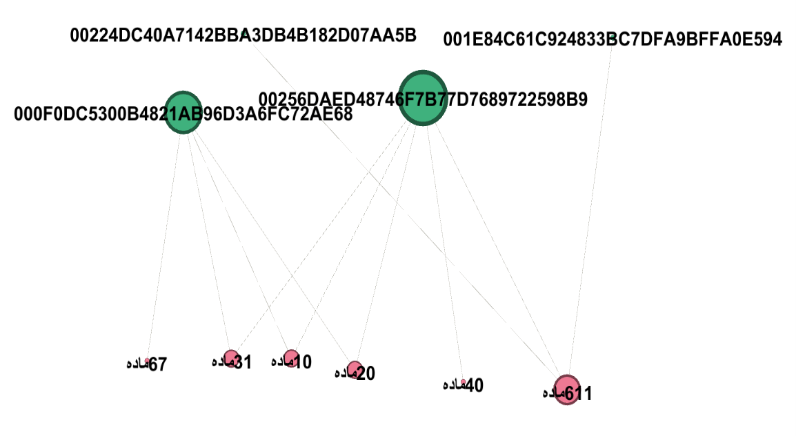
\includegraphics[scale=0.6]{Images/fig10}
		\vspace{-0.36cm}
		\caption{\footnotesize{Sample bipartite network connecting judicial rulings and legal articles}}\label{fig10}
	\end{center}
\end{figure}
\begin{figure}[!ht]
	\begin{center}
		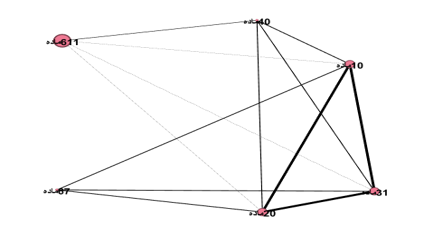
\includegraphics[scale=0.67]{Images/fig11}
		\vspace{-0.35cm}
		\caption{\footnotesize{Flattened legal-article network obtained from the bipartite graph}}\label{fig11}
	\end{center}\vspace{-0.3cm}
\end{figure}
\noindent Various analyses can be obtained by flattening a multipartite network. Generic legal articles may have high degree centrality but relatively weak edge weights because they co-occur with many different legal provisions. In contrast, domain-specific legal articles often exhibit stronger weighted connections due to frequent co-occurrence in judicial rulings. Such weighted relationships can support intelligent legal recommendation systems by suggesting legal articles that are commonly applied together.\\
In the flattened legal-article network, edges represent co-citation relationships among legal articles based on their joint occurrence in judicial rulings.
In the flattened legal-article network, centrality measures such as degree, betweenness, eigenvector, flow, information, harmonic, Katz, and PageRank are used to assess the structural importance of legal articles. Together, these metrics capture the influence, connectivity, accessibility, intermediary role, and information-flow characteristics of legal provisions within the legal citation network.

\begin{figure}[!ht]
	\begin{center}
		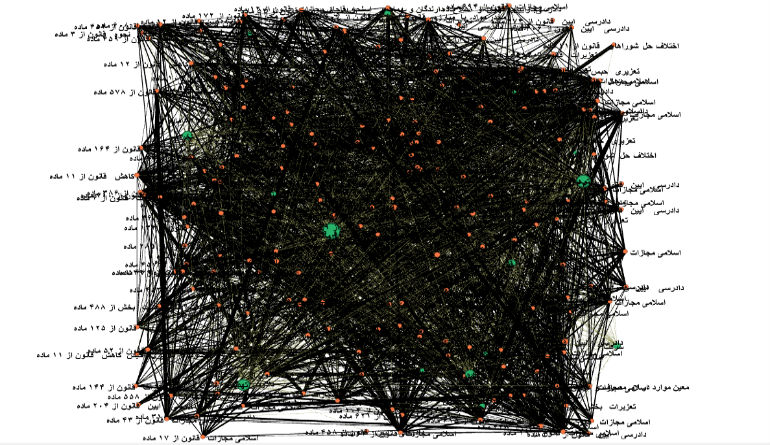
\includegraphics[scale=0.67]{Images/fig12}
		\vspace{-0.3cm}
		\caption{\footnotesize{Flattened network of legal articles derived from the bipartite graph of judicial rulings and legal articles}}\label{fig12}
	\end{center}
\end{figure}
\noindent Figure 5 illustrates the flattened charge-title network. In this representation, node size reflects the degree of a charge title, while edge weights indicate the frequency with which charge titles co-occur in judicial rulings. Similar to the legal-article network, centrality measures in this flattened charge-title network capture the relative importance, influence, and connectivity of charge titles within the legal system.

\begin{figure}[!ht]
	\begin{center}
		
\includegraphics[scale=0.67]{Images/fig13}
		\vspace{-0.3cm}
		\caption{\footnotesize{Flattened network of charge titles derived from the bipartite graph of judicial rulings and charge titles}}\label{fig13}
	\end{center}
\end{figure}
\noindent Similar to the flattened legal-article network, centrality measures in the flattened charge-title network are used to evaluate the structural importance, influence, connectivity, accessibility, and information-flow characteristics of charge titles within the legal network.

\subsection{Analysis and Implications of Complex Legal Networks}
The network analysis revealed that several legal documents and charge titles occupy central positions within the legal system. The tripartite representation uncovered direct and indirect relationships among judicial rulings, legal documents, and charge titles that are not evident in simple citation networks. Furthermore, betweenness centrality identified key intermediary nodes, while flattened networks revealed recurring co-occurrence patterns among legal articles and charge titles. These findings support judicial decision-making, legal recommendation systems, the identification of influential legal provisions, and similar-case retrieval \citep{Barron:2025}.
From a practical perspective, the proposed legal network can serve as a knowledge layer for intelligent judicial decision-support systems. By combining structural relationships among judicial rulings, legal articles, and charge titles, the network can assist judges in identifying relevant legal provisions, retrieving similar cases, and discovering frequently co-occurring legal articles during the preparation of judicial decisions. Moreover, the extracted network structure can support legal recommendation systems by prioritizing influential legal documents based on their structural importance rather than citation frequency alone. Such capabilities have the potential to improve the consistency of judicial reasoning, reduce legal research time, and enhance the transparency and explainability of AI-assisted legal decision-support systems.
\vspace{-0.3cm}
\section{	Conclusion}   
This study analyzed a Persian legal network using bipartite and tripartite graph representations. The results demonstrated that complex network analysis can identify influential legal entities and reveal key structural relationships within the legal system. Furthermore, natural language processing enabled the automatic extraction of legal documents and charge titles from judicial texts. Overall, the proposed framework demonstrates the potential of combining artificial intelligence and network analysis for legal analytics and judicial decision-support applications.
%%%%%%%%%%%%%%%%%%%%%%%% References %%%%%%%%%%%%%%%%%%%%%%%%%%%%%

\begin{thebibliography}{9}
\bibitem[Ahn et al. (2011)]{Ahn:2011}
Ahn Y.Y., Ahnert S.E., Bagrow J.P. and Barab\'{a}si A.L. (2011), Flavor network and the principles of food pairing, {\it Scientific Reports} 1(1), 196.

\bibitem[Barron et al. (2025)]{Barron:2025}
Barron R.C., Eren M.E., Serafimova O.M., Matuszek C. and Alexandrov B.S. (2025), Bridging legal knowledge and AI: retrieval-augmented generation with vector stores, knowledge graphs, and hierarchical non-negative matrix factorization, {\it arXiv preprint} arXiv:2502.20364.

\bibitem[Boulet et al. (2011)]{Boulet:2011}
Boulet R., Mazzega P. and Bourcier D. (2011), A network approach to the French system of legal codes---part I: analysis of a dense network, {\it Artificial Intelligence and Law} 19(4), 333--355.

\bibitem[Bourcier and Mazzega (2007)]{Bourcier:Mazzega:2007}
Bourcier D. and Mazzega P. (2007), Codification law article and graphs, {\it Legal Knowledge and Information Systems (JURIX 2007)}.

\bibitem[Chen et al. (2017)]{Chen:2017}
Chen Q., Hu Q., Huang J.X., He L. and An W. (2017), Enhancing recurrent neural networks with positional attention for question answering, {\it Proceedings of the 40th International ACM SIGIR Conference on Research and Development in Information Retrieval}, 993--996.

\bibitem[Chen et al. (2018a)]{Chen:2018a}
Chen Q., Hu Q., Huang J.X. and He L. (2018), CA-RNN: using context-aligned recurrent neural networks for modeling sentence similarity, {\it Proceedings of the AAAI Conference on Artificial Intelligence}.

\bibitem[Chen et al. (2018b)]{Chen:2018b}
Chen Q., Hu Q., Huang J.X. and He L. (2018), CAN: Enhancing sentence similarity modeling with collaborative and adversarial network, {\it Proceedings of the 41st International ACM SIGIR Conference on Research and Development in Information Retrieval}, 815--824.

\bibitem[Devlin et al. (2019)]{Devlin:2019}
Devlin J., Chang M.W., Lee K. and Toutanova K. (2019), BERT: Pre-training of deep bidirectional transformers for language understanding, {\it Proceedings of NAACL-HLT 2019}, 4171--4186.

\bibitem[Fosch-Villaronga (2022)]{FoschVillaronga:2022}
Fosch-Villaronga E. (Ed.) (2022), {\it Law and Artificial Intelligence: Regulating AI and Applying AI in Legal Practice}, TMC Asser Instituut.

\bibitem[Gong and Luo (2025)]{Gong:Luo:2025}
Gong S. and Luo X. (2025), DGGCCM: a hybrid neural model for legal event detection, {\it Artificial Intelligence and Law} 33(4), 1109--1149.

\bibitem[Gordon (2021)]{Gordon:2021}
Gordon J.S. (2021), AI and law: ethical, legal, and socio-political implications, {\it AI \& Society} 36(2), 403--404.

\bibitem[Guillaume and Latapy (2004)]{Guillaume:Latapy:2004}
Guillaume J.L. and Latapy M. (2004), Bipartite graphs as models of complex networks, {\it Workshop on Combinatorial and Algorithmic Aspects of Networking}.
	
\bibitem[Kamath et al. (2019)]{Kamath:2019}
Kamath S., Grau B. and Ma Y. (2019), Predicting and integrating expected answer types into a simple recurrent neural network model for answer sentence selection, {\it Computaci\'{o}n y Sistemas} 23(3), 665--673.

\bibitem[Laskar et al. (2019)]{Laskar:2019}
Laskar M.T.R., Hoque E. and Huang J.X. (2019), Utilizing bidirectional encoder representations from transformers for answer selection, {\it International Conference on Applied Mathematics, Modeling and Computational Science}.

\bibitem[Liu et al. (2019)]{Liu:2019}
Liu Y. et al. (2019), RoBERTa: A robustly optimized BERT pretraining approach, {\it arXiv preprint} arXiv:1907.11692.

\bibitem[Mayhew et al. (2020)]{Mayhew:2020}
Mayhew S., Nitish G. and Roth D. (2020), Robust named entity recognition with truecasing pretraining, {\it Proceedings of the AAAI Conference on Artificial Intelligence}.

\bibitem[Mikolov et al. (2013)]{Mikolov:2013}
Mikolov T., Chen K., Corrado G. and Dean J. (2013), Efficient estimation of word representations in vector space, {\it arXiv preprint} arXiv:1301.3781.

\bibitem[Newman et al. (2001)]{Newman:2001}
Newman M.E., Strogatz S.H. and Watts D.J. (2001), Random graphs with arbitrary degree distributions and their applications, {\it Physical Review E} 64(2), 026118.

\bibitem[Pennington et al. (2014)]{Pennington:2014}
Pennington J., Socher R. and Manning C.D. (2014), GloVe: Global vectors for word representation, {\it Proceedings of the 2014 Conference on Empirical Methods in Natural Language Processing (EMNLP)}, 1532--1543.

\bibitem[Rao et al. (2016)]{Rao:2016}
Rao J., He H. and Lin J. (2016), Noise-contrastive estimation for answer selection with deep neural networks, {\it Proceedings of the 25th ACM International Conference on Information and Knowledge Management (CIKM)}, 1913--1916.

\bibitem[Rao et al. (2019)]{Rao:2019}
Rao J., Liu L., Tay Y., Yang W., Shi P. and Lin J. (2019), Bridging the gap between relevance matching and semantic matching for short text similarity modeling, {\it Proceedings of the 2019 Conference on Empirical Methods in Natural Language Processing and the 9th International Joint Conference on Natural Language Processing (EMNLP-IJCNLP)}, 5370--5381.

\bibitem[Severyn and Moschitti (2013)]{Severyn:Moschitti:2013}
Severyn A. and Moschitti A. (2013), Automatic feature engineering for answer selection and extraction, {\it Proceedings of the 2013 Conference on Empirical Methods in Natural Language Processing (EMNLP)}, 458--467.

\bibitem[Siqueira et al. (2026)]{Siqueira:2026}
Siqueira F.A., Pressato D., Pereira F.S., da Silva N.F., Souza E., Dias M.S. and de Carvalho A.C. (2026), Segmenting Brazilian legislative text using weak supervision and active learning, {\it Artificial Intelligence \& Law} 34(1), 1.

\bibitem[Tarissan et al. (2013)]{Tarissan:2013}
Tarissan F., Quoitin B., M\'{e}rindol P., Donnet B., Pansiot J.J. and Latapy M. (2013), Towards a bipartite graph modeling of the internet topology, {\it Computer Networks} 57(11), 2331--2347.

\bibitem[Tay et al. (2017)]{Tay:2017}
Tay Y., Phan M.C., Tuan L.A. and Hui S.C. (2017), Learning to rank question answer pairs with holographic dual LSTM architecture, {\it Proceedings of the 40th International ACM SIGIR Conference on Research and Development in Information Retrieval}, 695--704.

\bibitem[Tumminello et al. (2011)]{Tumminello:2011}
Tumminello M., Miccich\'{e} S., Lillo F., Piilo J. and Mantegna R.N. (2011), Statistically validated networks in bipartite complex systems, {\it PLoS ONE} 6(3), e17994.

\bibitem[Vaswani et al. (2017)]{Vaswani:2017}
Vaswani A. et al. (2017), Attention is all you need, {\it Advances in Neural Information Processing Systems (NeurIPS)}.

\bibitem[Watts and Strogatz (1998)]{Watts:Strogatz:1998}
Watts D.J. and Strogatz S.H. (1998), Collective dynamics of small-world networks, {\it Nature} 393(6684), 440--442.

\bibitem[Yih et al. (2013)]{Yih:2013}
Yih W.T., Chang M.W., Meek C. and Pastusiak A. (2013), Question answering using enhanced lexical semantic models, {\it Proceedings of the 51st Annual Meeting of the Association for Computational Linguistics (ACL)}, 1744--1753.	
	
	
\end{thebibliography}
 \end{document}

